\begin{center}
	\Large\textbf{{{Сеточно-характеристический метод на неструктурированных расчётных сетках}}}
\end{center}

\section{Система уравнений}
В произвольной $D$-мерной области ($D = 2, 3$) решается система уравнений 
в частных производных гиперболического типа:
\begin{equation}
\label{general_equation}
	\frac{\partial\vec{u}}{\partial{t}}+
	\mathbf{A}_1\frac{\partial\vec{u}}{\partial{x_1}}+...+
	\mathbf{A}_D\frac{\partial\vec{u}}{\partial{x_D}}=0.
\end{equation}
Здесь $\{x_1, ..., x_D\}$ -- ортонормированный базис, 
$\vec{u} = \vec{u}(t, x_1, ..., x_D)$ -- вектор неизвестных размерности $N$,
матрицы $\mathbf{A}_i$ считаются постоянными по времени и пространству.
Кроме того, ставятся начальные условия -- значения $\vec{u}$ 
во всей области интегрирования в нулевой момент времени и
граничные условия -- некоторое количество скалярных условий на $\vec{u}$ 
на границе области интегрирования в любой момент времени.

Конкретный вид матриц и физический смысл уравнений можно не уточнять. 
Единственное условие -- матрицы должны быть диагонализуемы с полным набором 
собственных векторов, и для каждого ненулевого собственного значения должно быть
равное по модулю с противоположным знаком. Эти требования означают, фактически,
то, что система уравнений описывает некий волновой процесс. Количество
независимых скалярных граничных условий на $\vec{u}$ равно количеству
положительных (отрицательных) собственных значений матрицы $\mathbf{A}_i$, 
которое в дальнейшем обозначим за $M$.

Для более наглядной иллюстрации теоретических вопросов и 
демонстрации результатов будут использоваться волновые уравнения 
механики линейно-упругого тела и акустики. В виде \eqref{general_equation}
они выписаны в \cite{chelnokov}. Укажем здесь лишь состав переменных 
и основные свойства. 

При описании волновых процессов в упругом теле используются значения 
компонент скорости $\vec{v}$ и тензора напряжений $\sigma$.
В трёхмерном пространстве это составляет $N = 9$ независимых переменных:
\begin{equation}
	\vec{u} = (v_x,v_y,v_z,\sigma_{xx},\sigma_{xy},\sigma_{xz},\sigma_{yy},\sigma_{yz},\sigma_{zz})^{T}.
\end{equation}
Число положительных (отрицательных) собственных значений матрицы $\mathbf{A}_i$ 
в этом случае составляет $M = 3$, что соответствует 
одной продольной волне сжатия-разрежения (p-волна) и 
двум взаимно перпендикулярным поперечным волнам сдвига (s-волны).

В двумерном приближении число независимых переменных сокращается до $N = 5$:
\begin{equation}
	\vec{u} = (v_x,v_y,\sigma_{xx},\sigma_{xy},\sigma_{yy})^{T},
\end{equation}
а $M = 2$ -- одна p-волна и одна s-волна.

При описании волновых процессов в модели акустики независимо от размерности 
пространства $D$ число переменных в уравнении $N = D + 1$:
\begin{equation}
	\vec{u} = (v_1, ..., v_D, p)^T.
\end{equation}
Здесь $p$ -- давление, и $M = 1$ -- поперечные волны отсутствуют.


\section{Численный метод}
В наиболее общей постановке и с иллюстрацией множества приложений 
сеточно-характеристический метод (СХМ) 
изложен его создателями в \cite{magomedov_kholodov_1988}. 
К волновым уравнениям механики упругого тела 
СХМ впервые применён в \cite{petrov_kholodov}.
Основная идея реализации метода на неструктурированных расчётных сетках
предложена в \cite{magomedov_kholodov_1988}. 
Экономичная реализация граничных и контактных условий, а также
компактная запись аналитических формул спектрального разложения 
матриц $\mathbf{A}_i$ для моделей упругости и акустики предложены в \cite{chelnokov}.


\subsection{Неструктурированная расчётная сетка}
Для возможности применения метода к областям произвольной формы используются
треугольные и тетраэдральные неструктурированные расчётные сетки. 
Их построение осуществляется в основном с использованием 
библиотек CGAL \cite{cgal} и Ani3D \cite{ani3d}.
Значения искомой функции хранятся в узлах сетки. 

Подразумевается, что внутри каждой области интегрирования матрицы $\mathbf{A}_i$
постоянны. Для моделирования неоднородностей явно выделяются дополнительные
области интегрирования, между которыми рассчитывается контакт -- взаимозависимые
граничные условия для каждой из контактирующих областей.

Стоит отметить, что предложенный метод реализации граничных и контактных условий 
не закладывается на топологию ячейки сетки, то есть может быть применён, 
к примеру, и к октаэдральным расчётным сеткам.


\subsection{Расщепление по направлениям}
Поскольку классический СХМ рассматривает зависимость только от одной пространственной переменной,
для численного решения \eqref{general_equation} необходимо
перейти к решению одномерных систем уравнений -- так называемое расщепление по направлениям:
\begin{equation}
\label{equation_1d}
	\frac{\partial\vec{u}}{\partial{t}}+\mathbf{A_i}\frac{\partial\vec{u}}{\partial{\xi_i}} = 0, \quad i = 1 ... D.
\end{equation}
Здесь под $\{\xi_i\}$ подразумевается произвольный ортонормированный базис, 
не обязательно совпадающий с $\{x_i\}$ 
(вид матриц $\mathbf{A_i}$, конечно, меняется при смене базиса).

В данной работе используется предложенная в \cite{chelnokov}
экономичная по памяти и вычислительным ресурсам схема расщепления, 
обладающая при этом близким ко второму порядком точности по времени.
Полный шаг по времени $\tau$ решения многомерного уравнения \eqref{general_equation} 
состоит из $D$ последовательных ступеней. 
Каждая последовательная $i$-я ступень заключается в выполнении численного шага по времени
для $i$-го уравнения \eqref{equation_1d} на то же время $\tau$. 
В качестве значений старого временного слоя для $i$-й ступени 
берётся результат выполнения $(i-1)$-й, 
а результат выполнения последней ступени является решением 
многомерного уравнения на новом временном слое. 


\subsection{Решение одномерного уравнения}
По условию матрицы $\mathbf{A}_i$ диагонализуемы с полным набором собственных векторов:
\begin{equation}
	\label{diagonal_view}
	\mathbf{A} = \mathbf{U}^{-1}\mathbf{\Lambda}\mathbf{U}.
\end{equation}
Здесь $\mathbf{U}^{-1}$ -- матрица собственных векторов, 
$\mathbf{\Lambda}$ -- диагональная матрица собственных значений,
$\mathbf{U}$ -- матрица собственных строк.
Умножив \eqref{equation_1d} слева на $\mathbf{U}$, 
внеся постоянную матрицу $\mathbf{U}$ под знак дифференциала
и обозначая $\vec{r} = \mathbf{U}\vec{u}$ -- инварианты Римана, получаем:
\begin{equation}
	\label{in_riemann_invariants}
	\frac{\partial\vec{r}}{\partial{t}}+\mathbf{\Lambda}\frac{\partial\vec{r}}{\partial{x}} = 0.
\end{equation}
В новых переменных система распалась на независимые уравнения переноса.
Их численное решение заключается в интерполяции значения функции
на предыдущем временном слое в точке, где характеристика из узла 
на новом временном слое пересекает предыдущий. 
После переноса инвариантов с предыдущего временного слоя на новый
производится обратная замена переменных $\vec{u} = \mathbf{U}^{-1}\vec{r}$.

Для полностью одномерного случая 
сказанное проиллюстрировано на рисунке \ref{pic:gcm-idea}.
\begin{figure}[H]
	\center{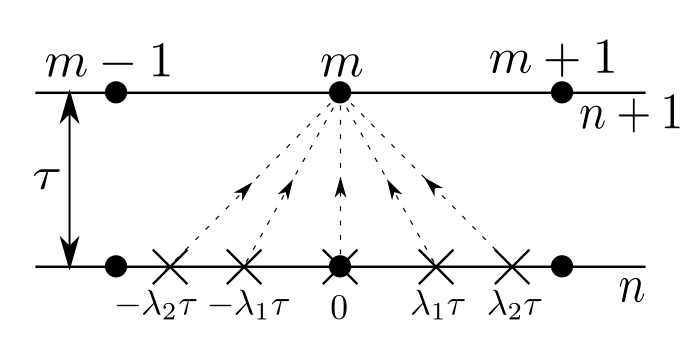
\includegraphics[width=0.5\textwidth]{pictures/gcm-idea.png}}
	\caption{Основная идея сеточно-характеристического метода}
	\label{pic:gcm-idea}
\end{figure}

Для многомерной (для наглядности $D = 2$) неструктурированной расчётной сетки 
идея расщепления по направлениям и переноса значений инвариантов Римана 
из точек пересечения их характеристик со старым временным слоем 
проиллюстрирована на рисунке \ref{pic:gcm-on-triangles}.
\begin{figure}[H]
	\center{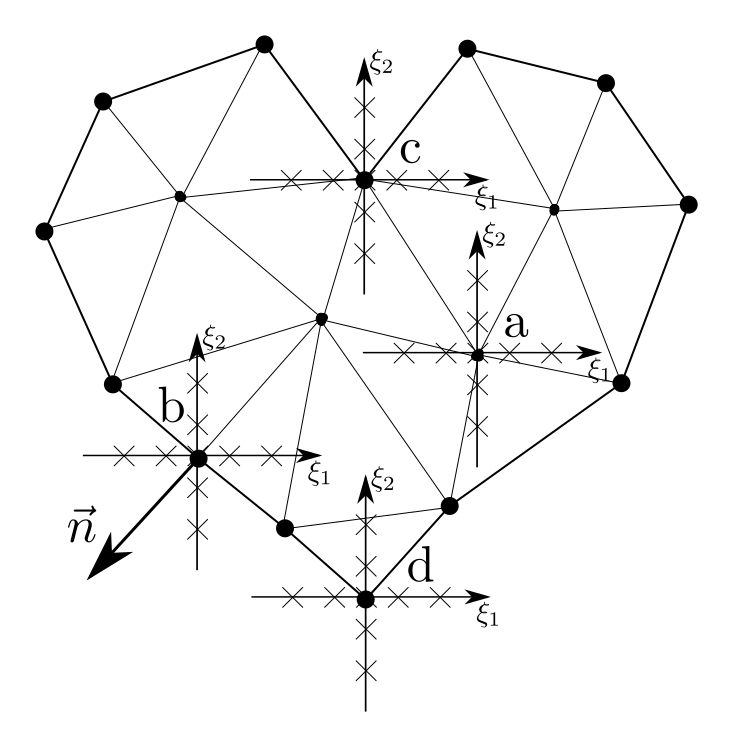
\includegraphics[width=0.5\textwidth]{pictures/gcm-on-triangles.png}}
	\caption{Иллюстрация сеточно-характеристического метода на треугольной расчётной сетке}
	\label{pic:gcm-on-triangles}
\end{figure}


\subsection{Метод на границе области интегрирования}
Описанный выше алгоритм пригоден для внутренних узлов, когда все выброшенные 
из узла характеристики пересекают предыдущий временной слой 
внутри области интегрирования, что соответствует случаю a) на рисунке \ref{pic:gcm-on-triangles}.

Для граничных и контактных узлов возможна ситуация, 
когда часть выпущенных из узла характеристик являются внешними, то есть
пересекают предыдущий временной слой вне области интегрирования -- 
случаи b), c) и d) на рисунке \ref{pic:gcm-on-triangles}.
При контакте двух областей интегрирования характеристика из узла
одной области может попадать в другую область. Тогда она также считается
внешней для своей области. В таких случаях применяется модификация алгоритма, 
называемая коррекцией внешними волнами. 

Поскольку часть характеристик выпадает за пределы области интегрирования 
и значения соответствующих им инвариантов Римана не могут быть интерполированы
и перенесены с предыдущего временного слоя, происходит, фактически, потеря информации. 
Однако в большинстве случаев эта информация может и должна быть восполнена
из заданных граничных и контактных условий.

Рассмотрим сначала случай b), когда число внешних характеристик 
равно числу независимых скалярных граничных условий $M$.


\subsubsection{Граница области интегрирования}
\paragraph{Общая форма записи граничного условия}
Произвольное линейное граничное условие для произвольной модели 
в общем виде записывается:
\begin{eqnarray}
\label{boundary_condition}
	\mathbf{B} \cdot \vec{u} = \vec{b}.
\end{eqnarray}
Здесь $\mathbf{B}$ -- матрица размерности $M \times N$, $\vec{b}$ -- вектор размерности $M$, 
определяющие собой конкретный вид граничного условия.

Рассмотрим для примера условие фиксированного напряжения $\vec{f}$, 
приложенного к полупространству с внешней нормалью $\vec{n}$ в модели упругого тела:
\begin{eqnarray}
\label{fixed_force}
	\mathbf{\sigma} \cdot \vec{n} = \vec{f}.
\end{eqnarray}
Примем для упрощения формул, что значение $\vec{f}$ указано в глобальном базисе,
тогда \eqref{fixed_force} в форме \eqref{boundary_condition} 
для трёхмерного случая запишется в виде: 
\begin{eqnarray}
	\vec{b} = \vec{f},
\end{eqnarray}
\begin{align}
\label{fixed_force_global_basis_3D}
	\mathbf{B} =
	\left( \begin{array}{cccccccccccc}
	 0 & 0 & 0 & n_x & n_y & n_z & 0 & 0 & 0 \\
	 0 & 0 & 0 & 0 & n_x & 0 & n_y & n_z & 0 \\
	 0 & 0 & 0 & 0 & 0 & n_x & 0 & n_y & n_z \\
	\end{array} \right).
\end{align}

Другой пример -- условие фиксированной нормальной скорости $v_n$ в модели акустики:
\begin{eqnarray}
	\vec{b} = (v_n),
\end{eqnarray}
\begin{align}
\label{fixed_normal_velocity_acoustic}
	\mathbf{B} =
	\left( \begin{array}{cccccccccccc}
	 \vec{n}^T, & 0 \\
	\end{array} \right).
\end{align}

\paragraph{Алгоритм расчёта граничных узлов}
\label{sec:good-border-case}
На первом этапе делается расчёт граничных узлов по алгоритму для внутренних, 
при этом все инварианты Римана, соответствующие внешним характеристикам, приравниваются к нулю. 
Получается $\vec{u}^{inner}$. Затем выполняется граничная коррекция -- 
добавление к результату такой линейной комбинации внешних волн, 
которая обеспечит выполнение граничного условия \eqref{boundary_condition}:
\begin{eqnarray}
	\mathbf{B} \cdot (\vec{u}^{inner} + \mathbf{\Omega} \cdot \vec{\alpha}) = \vec{b}.
\end{eqnarray}
Здесь $\mathbf{\Omega}$ -- матрица размерности $N \times M$, 
в столбцах которой стоят собственные векторы 
матрицы $\mathbf{A}$, соответствующие внешним характеристикам.
По физическому смыслу эти столбцы можно назвать внешними волнами,
то есть фиктивными волнами, как бы пришедшими извне области интегрирования.
Вектор $\vec{\alpha}$ размерности $M$ -- это вектор
коэффициентов линейной комбинации, которые нужно определить.

К примеру, если направление расчёта вдоль оси $x$, то 
для трёхмерной модели упругого тела матрица $\mathbf{\Omega}$ -- 
это три однонаправленных волны вдоль оси $x$:
\begin{align}
\label{Omega_for_elastic3D}
	\mathbf{\Omega} =
	\left( \begin{array}{cccccccccccc}
	-1 & 0  &  0 \\
	 0 & -1 &  0 \\
	 0 &  0 & -1 \\
	\frac{\lambda+2\mu}{c_p} & 0 & 0 \\
	0 & \frac{\mu}{c_s} & 0 \\
	0 & 0 & \frac{\mu}{c_s} \\
	\frac{\lambda}{c_p} & 0 & 0 \\
	0 & 0 & 0 \\
	\frac{\lambda}{c_p} & 0 & 0 \\
	\end{array} \right).
\end{align} 
Здесь первый столбец -- p-волна, далее -- две s-волны, 
$\lambda, \mu$ -- параметры Ламе, 
$c_p = \sqrt{\frac{\lambda + 2\mu}{\rho}}, c_s = \sqrt{\frac{\mu}{\rho}}$ -- 
скорости продольной и поперечной волн.

Другой пример: для модели акустики матрица $\mathbf{\Omega}$ состоит 
всего из одного столбца -- продольной волны вдоль направления расчёта. 
Если ввести обозначения $\vec{l}$ -- единичный вектор вдоль направления расчёта,
$c$ -- скорость продольной волны, $\rho$ -- плотность, то она запишется:
\begin{align}
\label{Omega_for_acoustic}
	\mathbf{\Omega} =
	\left( \begin{array}{cccccccccccc}
	 \vec{l} \\
	 c \rho \\
	\end{array} \right).
\end{align} 

Для определения $\vec{\alpha}$ необходимо решить 
СЛАУ с матрицей $\mathbf{B} \mathbf{\Omega}$ размерностью $M \times M$:
\begin{eqnarray}
\label{SLE_on_alpha}
	\mathbf{B} \mathbf{\Omega} \cdot \vec{\alpha} = \vec{b} - \mathbf{B} \cdot \vec{u}^{inner}.
\end{eqnarray}

После определения коэффициентов линейной комбинации производится собственно коррекция,
обеспечивающая выполнение граничных условий:
\begin{eqnarray}
\vec{u}^{n+1} = \vec{u}^{inner} + \mathbf{\Omega} \cdot \vec{\alpha}
\end{eqnarray}


\subsubsection{Контакт двух областей интегрирования}
\paragraph{Общая форма записи контактного условия}
Запись произвольного линейного контактного условия для произвольных моделей:
\begin{eqnarray}
\label{contact_condition}
\begin{split}
	\mathbf{B}_{1A} \cdot \vec{u}_A = \mathbf{B}_{1B} \cdot \vec{u}_B, \\
	\mathbf{B}_{2A} \cdot \vec{u}_A = \mathbf{B}_{2B} \cdot \vec{u}_B.
\end{split}
\end{eqnarray}
Здесь обозначения те же, что и в \eqref{boundary_condition}.

Для примера рассмотрим контактное условие полного слипания двух упругих тел.
Оно означает в точке контакта равенство скоростей:
\begin{eqnarray}
\vec{v}_A = \vec{v}_B
\end{eqnarray}
и равенство сил, действующих на контактную поверхность:
\begin{eqnarray}
\mathbf{\sigma}_A \cdot \vec{n} = \mathbf{\sigma}_B \cdot \vec{n},
\end{eqnarray}
где $\vec{n}$ -- нормаль к поверхности контакта. 
Все формулы записываются в глобальном базисе. 
Это означает, что в качестве $\mathbf{B}_{2A}$ и $\mathbf{B}_{2B}$ 
нужно взять матрицы для граничного условия фиксированного напряжения в глобальном базисе 
\eqref{fixed_force_global_basis_3D}, а в качестве 
$\mathbf{B}_{1A}$ и $\mathbf{B}_{1B}$ -- матрицы для граничного условия 
фиксированной скорости в глобальном базисе, 
которые здесь для краткости приводить не будем.

Другой пример -- скольжение двух тел в модели акустики -- 
означает равенство компонент скорости вдоль направления контакта:
\begin{eqnarray}
\vec{v}_A \cdot \vec{n} = \vec{v}_B \cdot \vec{n}
\end{eqnarray}
и равенство давлений:
\begin{eqnarray}
p_A = p_B.
\end{eqnarray}
Здесь также в качестве матриц $\mathbf{B}$ из \eqref{contact_condition} 
используются матрицы для линейных граничных условий, в том числе 
\eqref{fixed_normal_velocity_acoustic}.


\paragraph{Алгоритм расчёта контактных узлов}
\label{sec:good-contact-case}
Все действия аналогичны расчёту граничных узлов. 
Сначала делается расчёт контактных узлов в обоих телах по алгоритму для внутренних.
Получается ${\vec{u}_A}^{inner}$ и ${\vec{u}_B}^{inner}$. 
Затем выполняется контактная коррекция -- 
добавление в обоих узлах такой линейной комбинации внешних волн, 
которая обеспечит выполнение контактного условия \eqref{contact_condition}. 

Распишем сообразно сказанному условие \eqref{contact_condition}:
\begin{eqnarray}
	\mathbf{B}_{1A} \cdot ({\vec{u}_A}^{inner} + \mathbf{\Omega}_A \cdot \vec{\alpha}_A) = \mathbf{B}_{1B} \cdot ({\vec{u}_B}^{inner} + \mathbf{\Omega}_B \cdot \vec{\alpha}_B), \\
\label{second_line_in_contact_condition_wide}
	\mathbf{B}_{2A} \cdot ({\vec{u}_A}^{inner} + \mathbf{\Omega}_A \cdot \vec{\alpha}_A) = \mathbf{B}_{2B} \cdot ({\vec{u}_B}^{inner} + \mathbf{\Omega}_B \cdot \vec{\alpha}_B).
\end{eqnarray}

Раскроем скобки:
\begin{eqnarray}
	(\mathbf{B}_{1A} \mathbf{\Omega}_A) \cdot  \vec{\alpha}_A = \mathbf{B}_{1B} \cdot {\vec{u}_B}^{inner} - \mathbf{B}_{1A} \cdot {\vec{u}_A}^{inner} + (\mathbf{B}_{1B} \mathbf{\Omega}_B) \cdot \vec{\alpha}_B
\end{eqnarray}

Сделаем переобозначения:
\begin{align}
\label{matrixRcontact}
\mathbf{R} &= (\mathbf{B}_{1A} \mathbf{\Omega}_A)^{-1}, &\\
\vec{p} &= \mathbf{R} \cdot (\mathbf{B}_{1B} \cdot {\vec{u}_B}^{inner} - \mathbf{B}_{1A} \cdot {\vec{u}_A}^{inner}), &\\
\mathbf{Q} &= \mathbf{R} \cdot (\mathbf{B}_{1B} \mathbf{\Omega}_B).
\end{align}

Тогда:
\begin{eqnarray}
\label{alpha_A_from_B}
\vec{\alpha}_A = \vec{p} + \mathbf{Q} \cdot \vec{\alpha}_B.
\end{eqnarray}

Подставим в \eqref{second_line_in_contact_condition_wide}:
\begin{eqnarray}
\begin{split}
\mathbf{B}_{2A} \cdot {\vec{u}_A}^{inner} + (\mathbf{B}_{2A} \mathbf{\Omega}_A) \cdot \vec{p} + (\mathbf{B}_{2A} \mathbf{\Omega}_A) \cdot \mathbf{Q} \cdot \vec{\alpha}_B = \\ =
\mathbf{B}_{2B} \cdot {\vec{u}_B}^{inner} + (\mathbf{B}_{2B} \mathbf{\Omega}_B) \cdot \vec{\alpha}_B.
\end{split}
\end{eqnarray}

Получим СЛАУ на $\vec{\alpha}_B$:
\begin{eqnarray}
\label{SLE_on_alphaB}
\begin{split}
\Bigg[  (\mathbf{B}_{2B} \mathbf{\Omega}_B) - (\mathbf{B}_{2A} \mathbf{\Omega}_A) \cdot \mathbf{Q}  \Bigg] \cdot \vec{\alpha}_B = \\ = 
(\mathbf{B}_{2A} \mathbf{\Omega}_A) \cdot \vec{p} + \mathbf{B}_{2A} \cdot {\vec{u}_A}^{inner} - \mathbf{B}_{2B} \cdot {\vec{u}_B}^{inner}.
\end{split}
\end{eqnarray}

Решив систему на $\vec{\alpha}_B$, находим $\vec{\alpha}_A$ из \eqref{alpha_A_from_B}.

После чего производится собственно коррекция, обеспечивающая выполнение контактных условий:
\begin{eqnarray}
{\vec{u}_A}^{n+1} = {\vec{u}_A}^{inner} + \mathbf{\Omega}_A \cdot \vec{\alpha}_A, \\
{\vec{u}_B}^{n+1} = {\vec{u}_B}^{inner} + \mathbf{\Omega}_B \cdot \vec{\alpha}_B
\end{eqnarray}


\subsection{Вырождение матриц СЛАУ граничного и контактного корректора}
\subsubsection{Описание проблемы}
\label{degeneration_problem}
Итак, расчёт граничных узлов по алгоритму \ref{sec:good-border-case} 
требует решения СЛАУ \ref{SLE_on_alpha}, 
расчёт контактных узлов по алгоритму \ref{sec:good-contact-case} требует 
решения СЛАУ \ref{SLE_on_alphaB} и обращения матрицы \ref{matrixRcontact}.
Размерность матриц во все трёх случаях равна $M \times M$, 
то есть относительно небольшая: для уравнений упругости в $D$-мерном 
пространстве размерность $D \times D$, что даёт возможность 
использовать правило Крамера и другие аналитические формулы, 
для уравнений акустики размерность $1 \times 1$. 

Однако это не снимает вопрос о возможности вырождения этих матриц. 
Для иллюстрации рассмотрим расчёт граничного узла в трёхмерной 
модели упругого тела при условии фиксированного напряжения на границе. 
Все матрицы, необходимые для расчёта по формуле \ref{SLE_on_alpha}, уже выписаны: 
матрица $\mathbf{B}$ в \ref{fixed_force_global_basis_3D} и 
матрица $\mathbf{\Omega}$ в \ref{Omega_for_elastic3D}. 
Остаётся их перемножить:
\begin{align}
	\mathbf{B} \mathbf{\Omega} = \frac{1}{c_1 c_2}
	\left( \begin{array}{cccccccccccc}
	 (\lambda + 2\mu) n_x c_2 & \mu n_y c_1 & \mu n_z c_1   \\
	 \lambda n_y c_2          & \mu n_x c_1 & 0             \\
	 \lambda n_z c_2          & 0 & \mu n_x c_1             \\
	\end{array} \right)
\end{align}
и взять определитель:
\begin{eqnarray}
	\det (\mathbf{B} \mathbf{\Omega}) = \frac{\mu^{2}}{c_1 c^2_2} \cdot n_x \cdot (2 (\lambda + \mu) n^2_x - \lambda).
\end{eqnarray}
Введя обозначение $\nu$ -- коэффициент Пуассона, из условия 
$\det (\mathbf{B} \mathbf{\Omega}) = 0$ получаем:
\begin{eqnarray}
\left[
\begin{gathered} 
	 n_x = 0  \hfill  \\
	 n^2_x = \frac{\lambda}{2(\lambda + \mu)} \equiv \nu < \frac{1}{2}, \hfill  \\
\end{gathered} 
\right.
\end{eqnarray}
Здесь направление расчёта выбиралось вдоль оси $x$, в то время как нормаль 
к границе была произвольной. Очевидно, что для обобщения условия 
вырождения для произвольного направления расчёта $\vec{l}$ нужно $n_x$ заменить на 
$(\vec{n} \cdot \vec{l})$.

Аналогично для модели акустики и граничного условия фиксированной 
нормальной скорости с учётом \ref{fixed_normal_velocity_acoustic} 
и \ref{Omega_for_acoustic} получаем:
\begin{eqnarray}
\label{BOmega_acoustic}
	\det (\mathbf{B} \mathbf{\Omega}) = \mathbf{B} \mathbf{\Omega} = (\vec{n} \cdot \vec{l}).
\end{eqnarray}

Условия вырождения матриц СЛАУ граничного корректора для обеих моделей и 
двух типов граничных условий сведены в таблицу:
\begin{center}
    \begin{tabular}{ | l | l | l | }
    \hline
    Модель & Фиксированная сила & Фиксированная скорость \\ \hline
    Упругость 3D & $\left[ \begin{gathered} (\vec{n} \cdot \vec{l}) = 0  \hfill \\ (\vec{n} \cdot \vec{l})^2 = \nu \hfill \\ \end{gathered} \right.$
 & - \\ \hline
    Упругость 2D & $(\vec{n} \cdot \vec{l})^2 = \nu$ & -  \\ \hline
    Акустика & - & $(\vec{n} \cdot \vec{l}) = 0$     \\ \hline
    \end{tabular}
\end{center}

Можно сделать следующие выводы. 
Во-первых, вырождение матриц граничного и контактного корректоров возможно. 
Во-вторых, оно далеко не всегда связано с перпендикулярностью направления 
расчёта и нормали, как это могло бы показаться. 
В-третьих, можно отметить, что вырождение возможно только тогда, 
когда в запись граничного условия так или иначе входит значение нормали.

График на рисунке \ref{pic:corrector_conditional} показывает рассчитанные 
значения определителя и числа обусловленности в случаях 
фиксированного напряжения для трёхмерных уравнений упругости и 
фиксированной нормальной скорости для уравнений акустики. 
\begin{figure}[H]
	\center{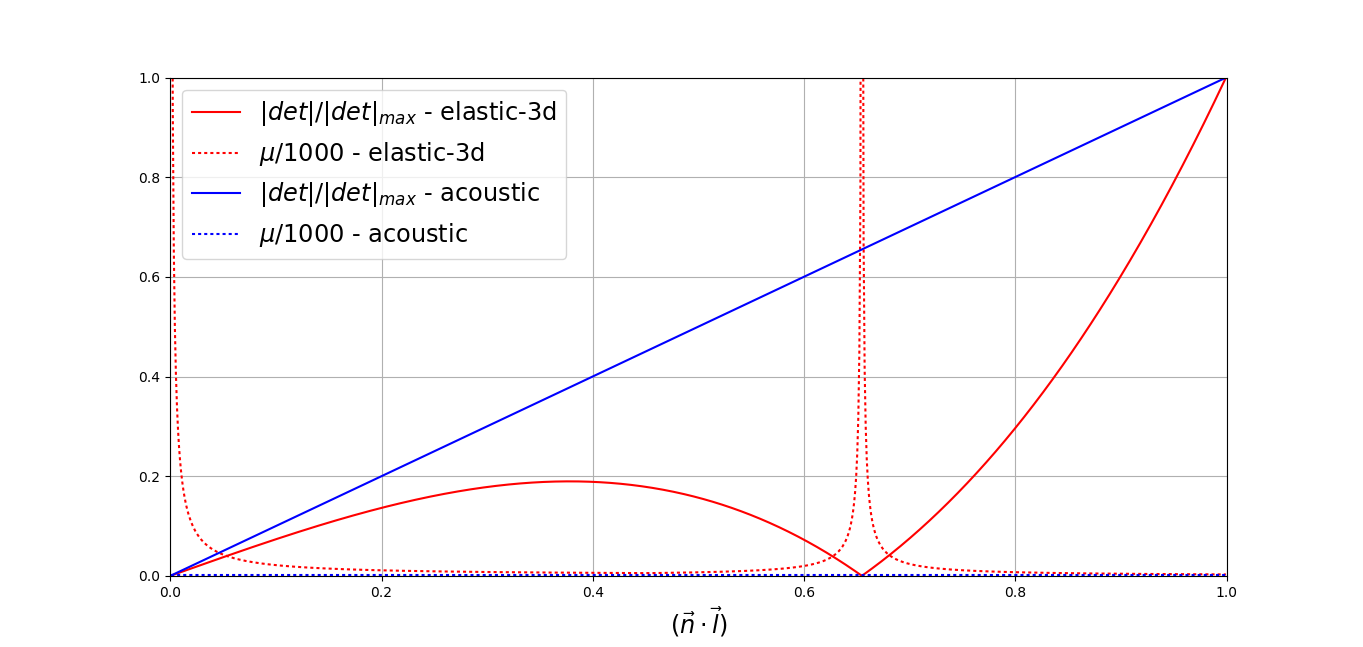
\includegraphics[width=0.8\textwidth]{pictures/corrector_conditional.png}}
	\caption{К вопросу вырождения матриц граничного корректора}
	\label{pic:corrector_conditional}
\end{figure}

Игнорирование возможности вырождения матриц граничного и контактного 
корректоров приводит к неустойчивости метода: значения искомой функции 
$\vec{u}$ вблизи границы области интегрирования неограниченно возрастают. 
Для стабилизации необходимы дополнительные усилия.


\subsubsection{Контроль определителя и согласованности начальных и граничных условий}
Первое очевидное действие -- проверка определителя матрицы на близость к нулю. 
Для двумерной и трёхмерной моделей упругости приближение к нулю определителя 
сопровождается резким ростом числа обусловленности, и с определённого момента 
точность решения СЛАУ становится неприемлемой. Для модели акустики, где размерность 
``матрицы'' $1 \times 1$, понятие числа обусловленности теряет смысл, но,
тем не менее, необходимо отсечь возможность деления на ноль. 

Итак, при достаточной близости детерминанта к нулю нельзя производить 
коррекцию по изложенной схеме. Означает ли это, что, 
если в таких случаях вообще не производить коррекцию, 
граничные или контактные условия по итогам ступени расчёта не будут выполнены? 

Когда в \ref{degeneration_problem} изучается вырожденность матрицы 
граничного корректора, фактически ищется ответ на вопрос, насколько линейная 
комбинация внешних волн может повлиять на выполнение граничного условия. 
Заметим, что ``внешние'' волны -- это однонаправленные волны вдоль направления расчёта, 
характеристики которых приходят в расчётный узел извне области интегрирования. 
В противовес им можно выделить ``внутренние'' -- те, что приходят изнутри области.
Также заметим, что при выкладках в \ref{degeneration_problem} тот факт, что комбинация 
волн является именно ``внешней'', а не ``внутренней'', не имеет значения. 
Отсюда ясно, что обусловленность матрицы граничного корректора показывает не только 
возможность влияния комбинации внешних волн на выполнение граничного условия, но и 
вообще возможность любых волн вдоль этого направления изменять граничные условия данного типа. 

Другими словами, если вдоль данного направления 
с помощью внешних волн невозможно повлиять на выполнение или невыполнение 
граничных условий, то и внутренние волны тоже не могут их нарушить.
А значит, если граничные условия в узле уже были выполнены до внутреннего этапа расчёта, то 
они останутся выполненными и после него, и граничная коррекция не нужна.

Отсюда очевидна необходимая модификация метода. Перед внутренним этапом расчёта 
граничного узла значения вектора решения $\vec{u}$ в нём сразу ``поправляются'' так, чтобы выполнялись 
граничные условия. Причём если граничные условия зависят от времени, то выставляются 
значения, соответствующие новому, а не текущему, временному слою. Это обеспечивает условие 
устойчивости метода на границе: на каждой ступени расчёта граничная коррекция производится лишь в том 
объёме, в котором внутренний этап этой ступени мог нарушить выполнение граничных условий.

Осталось уточнить слово ``поправляются'', специально использованное, 
чтобы отличить эту процедуру от граничной коррекции. 
Поскольку число независимых скалярных граничных условий на вектор решения $M$
всегда меньше его размерности $N$, поменять его значения так, чтобы эти условия  
удовлетворялись, можно бесконечным числом способов, 
в том числе той же граничной коррекцией. В данном случае делается следующее. 
Граничные и контактные условия, как правило, определяют некоторые значения 
вектора решения $\vec{u}$ в локальном базисе, связанном с граничной или контактной поверхностью. 
Это может быть, к примеру, нормальная к границе области компонента скорости или 
вектор напряжения, действующего на граничную поверхность. Поэтому наиболее логичным 
представляется перевести значения $\vec{u}$ в локальный базис, после чего 
выставить необходимые значения согласно граничным условиям, а затем перейти 
обратно в глобальный базис. Из всех прочих эта процедура 
оказывает минимальное влияние на значения вектора решения $\vec{u}$. 

На рисунке \ref{pic:fixed-normal-velocity} проведённые рассуждения иллюстрируются для 
уравнений акустики и граничного условия фиксированной нормальной скорости $v_n$. 
Вдоль оси $\xi_i$ с точностью до множителя могут распространятся только два типа волн:
$\{ \vec{v}_1, - p_1 \}$ -- сонаправленная с осью $\xi_i$ и 
$\{ \vec{v}_1, p_1 \}$ -- против оси $\xi_i$. 
Возможность этих волн повлиять на нормальную компоненту скорости тем меньше, чем 
ближе угол между нормалью и направлением расчёта к $\pi/2$, что и отражает условие 
\ref{BOmega_acoustic}. Поэтому чем меньше $(\vec{n} \cdot \xi_i)$, тем большая амплитуда 
внешней волны требуется для удовлетворения граничного условия $(\vec{v} \cdot \vec{n}) = v_n$. 
С другой стороны, волна, пришедшая изнутри, влияет на граничное условие не сильнее внешней. 
Поэтому, если ещё до внутреннего этапа расчёта значение нормальной скорости в узле 
было выставлено согласно граничным условиям, то и величина граничной коррекции будет 
адекватна величине изменения граничного условия на внутреннем этапе расчёта.

\begin{figure}[H]
	\center{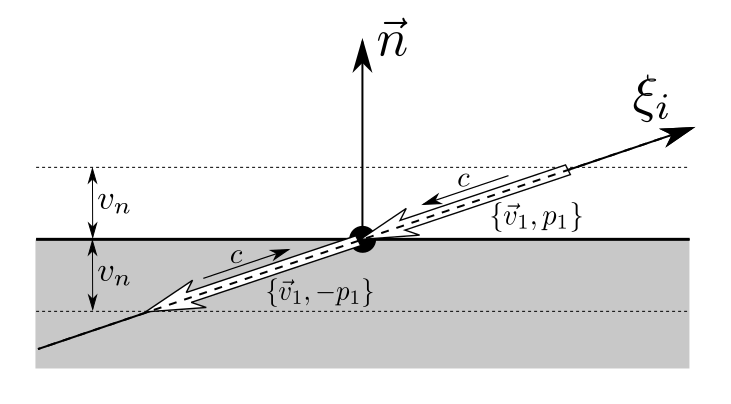
\includegraphics[width=0.8\textwidth]{pictures/fixed-normal-velocity.png}}
	\caption{К пояснению возможности влияния волн вдоль направления расчёта на выполнение граничных условий}
	\label{pic:fixed-normal-velocity}
\end{figure}

Таким образом, возможность вырождения матриц граничного и контактного корректоров 
требует особого алгоритма и его тонкой настройки на предмет критических значений определителя, 
но не представляет неразрешимую для метода проблему.


\subsubsection{Сложные случаи на границе областей интегрирования}
\label{bad_border_cases}
В случае b) на рисунке \ref{pic:gcm-on-triangles} 
количество внешних характеристик для граничного узла равняется количеству независимых 
скалярных граничных условий. Это означает, с одной стороны, 
что вся потерянная в результате выпада характеристик из области интегрирования информация 
компенсируется за счёт граничных условий, а с другой, 
что имеется достаточное количество внешних волн для выполнения граничной коррекции. 
При ступени расчёта вдоль направления $\xi_1$ варианты c) и d) 
существенно отличаются от b) тем, что  
в c) отсутствуют внешние волны, с помощью которых была бы возможна граничная коррекция, 
а в d), напротив, число внешних волн превышает число граничных условий, что 
приводит к неизбежной потери информации. В этих случаях имеет смысл говорить не о 
``внешних'' и ``внутренних'' волнах, а о ``правых'' и ``левых'', в зависимости от 
того, с какой стороны волны приходят в узел вдоль направления расчёта.

Численные эксперименты показали, что для обоих вариантов c) и d) устойчивой является 
следующая модификация метода. 
Сначала по общему для всех узлов алгоритму ``подправляются'' под 
граничные условия значения вектора решения и делается внутренний этап расчёта. 
Затем рассчитываются два варианта граничной коррекции: с помощью ``правых'' и 
с помощью ``левых'' групп волн. После чего берётся их полусумма. 

Можно было бы возразить, что в варианте c) нет выпавших вне области характеристик, 
поэтому коррекцию вообще проводить не нужно. Однако граничное условие на внутреннем этапе расчёта 
могло быть нарушено, а следовательно, коррекция необходима, иначе не будут  
согласованны граничные и начальные условия на следующей ступени расчёта.

Аналогичные сложности и способы их преодоления существуют и при расчёте контактов двух областей. 

Отметим, что предложенные решения являются на самом деле довольно искуственными, 
и не решают упомянутой проблемы потери информации. На практике это оборачивается тем, 
что на существенно неструктурированных расчётных сетках в местах, где реализуются 
описанные сложности, возникают нефизичные возмущения, не убывающие по времени. 
И это, в отличии от проблемы вырождения матриц корректоров, является принципиальным 
ограничением метода, связанным в первую очередь с расщеплением по направлениям.

Единственным известным автору средством сглаживания этого эффекта является 
использование нового базиса $\{\xi_i\}$ на каждом шагу по времени, благодаря 
чему в проблемных местах сетки 
возмущения всё же не накапливаются от шага к шагу и не нарастают экспоненциально.

Отдельную проблему представляют случаи контакта в одном узле 
трёх и более областей интегрирования. Поскольку ограничения на 
число контактирующих в одном узле тел нет, 
прямой учёт контакта всех областей потребовал бы чересчур тяжёлого алгоритма. 
В качестве компромисса между сложностью и обоснованностью метода можно предложить 
расчёт многоконтактного узла просто как граничного для каждой контактирующей области. 


\subsection{Некурантовский шаг по времени}
\subsubsection{Необходимость расчёта с шагом больше курантовского в 3D}
На графиках на рисунке \ref{fig:cell_h_histograms} представлены распределения значений высот 
треугольников в двумерных и тетраэдров в трёхмерных типичных неструктурированных сетках. 
Можно видеть принципиальное различие, заключающееся в том, что для треугольной сетки 
минимальная высота составляет примерно половину средней высоты, 
в то время как для тетраэдральной сетки различие минимальной и средних высот 
составляет несколько порядков, причём вырожденные ячейки представляют 
собой не единичные выбросы, а вполне систематическое явление.
\begin{figure}[H]
\centering
\begin{subfigure}{.5\textwidth}
  \centering
  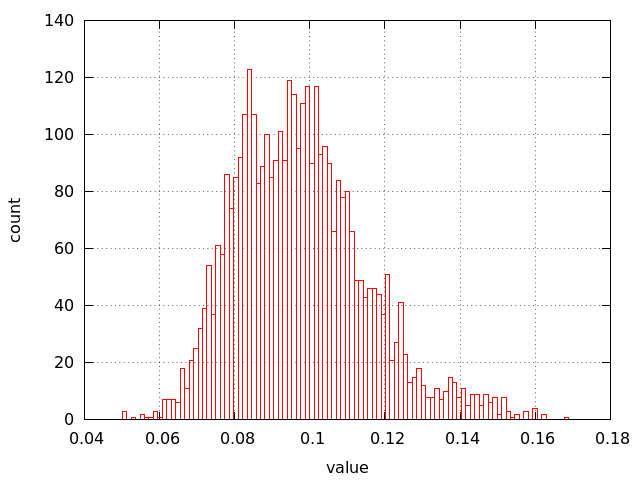
\includegraphics[width=1.0\linewidth]{pictures/cells_heights_histogram_2d.png}
  \caption{2D}
  \label{fig:hist-2d}
\end{subfigure}%
\begin{subfigure}{.5\textwidth}
  \centering
  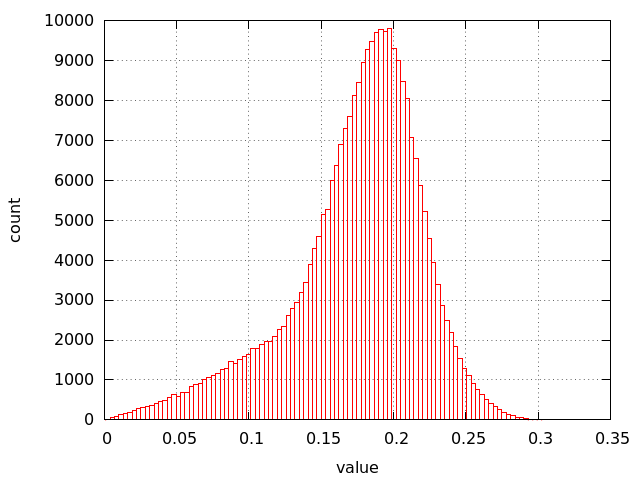
\includegraphics[width=1.0\linewidth]{pictures/cells_heights_histogram_3d.png}
  \caption{3D}
  \label{fig:hist-3d}
\end{subfigure}
\caption{Гистограммы значений высот ячеек типичных неструктурированных сеток}
\label{fig:cell_h_histograms}
\end{figure}

По аналогии с численными методами на регулярных расчётных сетках 
для неструктурированных сеток также можно ввести понятие условия Куранта 
на шаг по времени:
\begin{eqnarray}
\label{courant_condition}
	\frac{c_{max} \tau}{h_{min}} < 1.
\end{eqnarray}
Здесь под $h_{min}$ понимается минимальная высота ячейки. Отметим, что 
все предыдущие рассуждения велись в предположении, что это условие выполнено.

Однако из рисунка \ref{fig:cell_h_histograms} очевидно, что, в отличии от двумерных, 
для трёхмерных неструктурированных сеток условие Куранта в таком виде невыполнимо 
из-за вырожденных ячеек. Можно предложить следующие пути решения проблемы:
\begin{itemize}
\item Применение для построения расчётных сеток специальных алгоритмов генерации, 
которые обеспечат приемлемую минимальную высоту ячейки
\item Применение так называемых иерархических шагов по времени, когда в местах 
малой высоты ячеек используется дробный до нужной малости шаг по времени
\item Расчёт с шагом, определяемым \ref{courant_condition}, где в качестве $h_{min}$ 
берётся не минимальная, а средняя или иная приемлемая высота ячейки
\end{itemize}

Осуществимость первых двух подходов автором подробно не исследовалась, 
вместе с тем очевидно, что на пути их реализации будут существенные трудности. 
В данной работе применяется третий подход, в котором величина шага по времени 
регулируется объективной мелкостью расчётной сетки. Интерполяция значения функции 
на предыдущем временном слое производится при этом, естественно, по той ячейке, 
в которую попала характеристика, а не по ближайшей к рассчитываемому узлу, поэтому 
правило Куранта -- интерполяция по области зависимости решения -- 
не нарушается, а численные эксперименты доказывают устойчивость такого метода.


\subsubsection{Возникающие в связи с этим сложности}
Однако при всей простоте у выбранного подхода существует очевидная проблема. 
\begin{figure}[H]
	\center{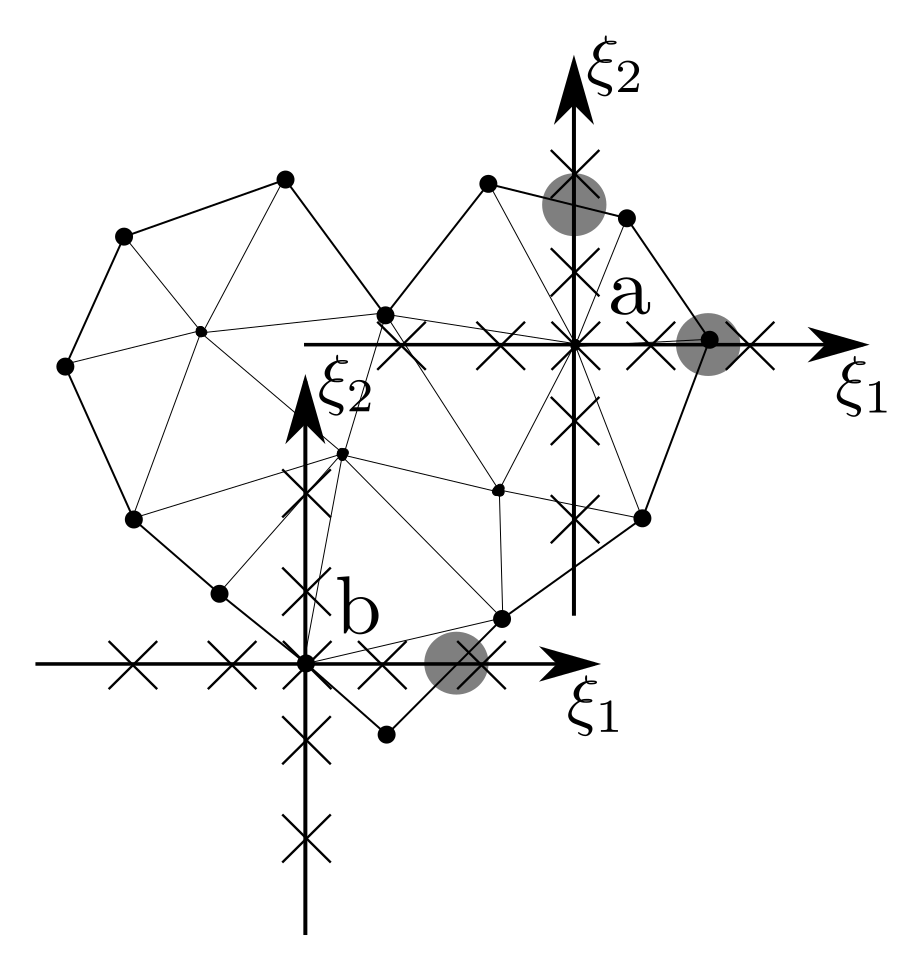
\includegraphics[width=0.5\textwidth]{pictures/gcm-on-triangles-non-courant.png}}
	\caption{Выпадения внутренних характеристик из области интегрирования отмечены серым}
	\label{pic:gcm-on-triangles-non-courant}
\end{figure}
Расстояние между узлом и точкой, в которой производится интерполяция, 
превосходит минимальную высоту ячейки. Поэтому внешние характеристики могут 
появляться не только у граничных узлов, но и у внутренних 
(вариант a) на рисунке \ref{pic:gcm-on-triangles-non-courant}). 

Модификация метода для внутренних узлов на такой случай 
была предложена ещё в \cite{magomedov_kholodov_1988}. Она заключается в том, 
что инвариант Римана для характеристики, пересекающей границу области интегрирования, 
интерполируется не на предыдущем временном слое, а в пространстве-времени между двумя 
слоями с использованием значений в ближайших к точке пересечения граничных узлах 
на текущем и на новом временных слоях. Граничные узлы при таком подходе, 
естественно, должны быть рассчитаны до внутренних.

У граничных же узлов в достаточно выпуклых углах области интегрирования характеристики, 
проходя сначала через внутренность области, могут пересекать затем её границу 
и оказываться внешними. Поэтому у граничного узла может быть, фактически, 
произвольный набор внешних характеристик 
(вариант b) на рисунке \ref{pic:gcm-on-triangles-non-courant}). 
Так же, как и в случаях, описанных в разделе \ref{bad_border_cases}, 
это приводит к потери информации и нефизичным возмущениям. Применить 
интерполяцию в пространстве-времени в данном случае нельзя, поскольку 
нет гарантии, что граничные узлы, по которым должна проводиться интерполяция, 
уже посчитаны на следующем временном слое. 

Можно предложить альтернативный метод: рассчитать значение функции в точке пересечения 
характеристики с границей как во вспомогательном узле, 
расположенном между временными слоями, и посчитать затем нужное значение 
инварианта Римана, который переносится из этой точки в расчётный узел. 
Возможно, придётся применить эту процедуру рекурсивно, 
пока все внутренние характеристики из вспомогательных узлов не попадут внутрь 
области интегрирования. 


\section{Результаты}
Череп, данные по количеству узлов, ячеек, узлов на слой


\section{Заключение}
 принципиальное ограничение метода 
Рассуждения в пользу методов с ячейками и потоками для нестр. сеток


\section{Дополнения}
\subsection{Интерполяция второго порядка на неструктурированной сетке }
\subsection{Стабильный алгоритм поиска 
ячейки пересечения характеристики с предыдущим временным слоем}


\begin{thebibliography}{99}
\addcontentsline{toc}{section}{Литература}

\bibitem{magomedov_kholodov_1988} Магомедов К.М., Холодов А.С. 
Сеточно-характеристические численные методы. — М.: Наука, 1988, 288 с.

\bibitem{petrov_kholodov} Петров И.Б., Холодов А.С. 
Численное исследование некоторых динамических задач механики деформируемого 
твёрдого тела сеточно-характеристическим методом, 
Ж. вычисл. матем. и матем. физ., 24:5 (1984), 722–739.

\bibitem{chelnokov} Челноков Ф.Б., Явное представление 
сеточно-характеристических схем для уравнений упругости в двумерном и
 трехмерном пространствах, Матем. моделирование, 18:6 (2006), 96–108.

\bibitem{cgal} CGAL, Computational Geometry Algorithms Library, http://www.cgal.org

\bibitem{ani3d} 3D generator of anisotropic meshes http://sourceforge.net/projects/ani3d

\end{thebibliography}














